\documentclass{fkssolpub}

\usepackage[czech]{babel}
\usepackage{fontspec}
\usepackage{fkssugar}
\usepackage{amsmath}
\usepackage{graphicx}

\author{Ondřej Sedláček}
\school{Gymnázium Oty Pavla} 
\series{3s}
\problem{1} 

\begin{document} 

\begin{figure}
  \begin{center}
    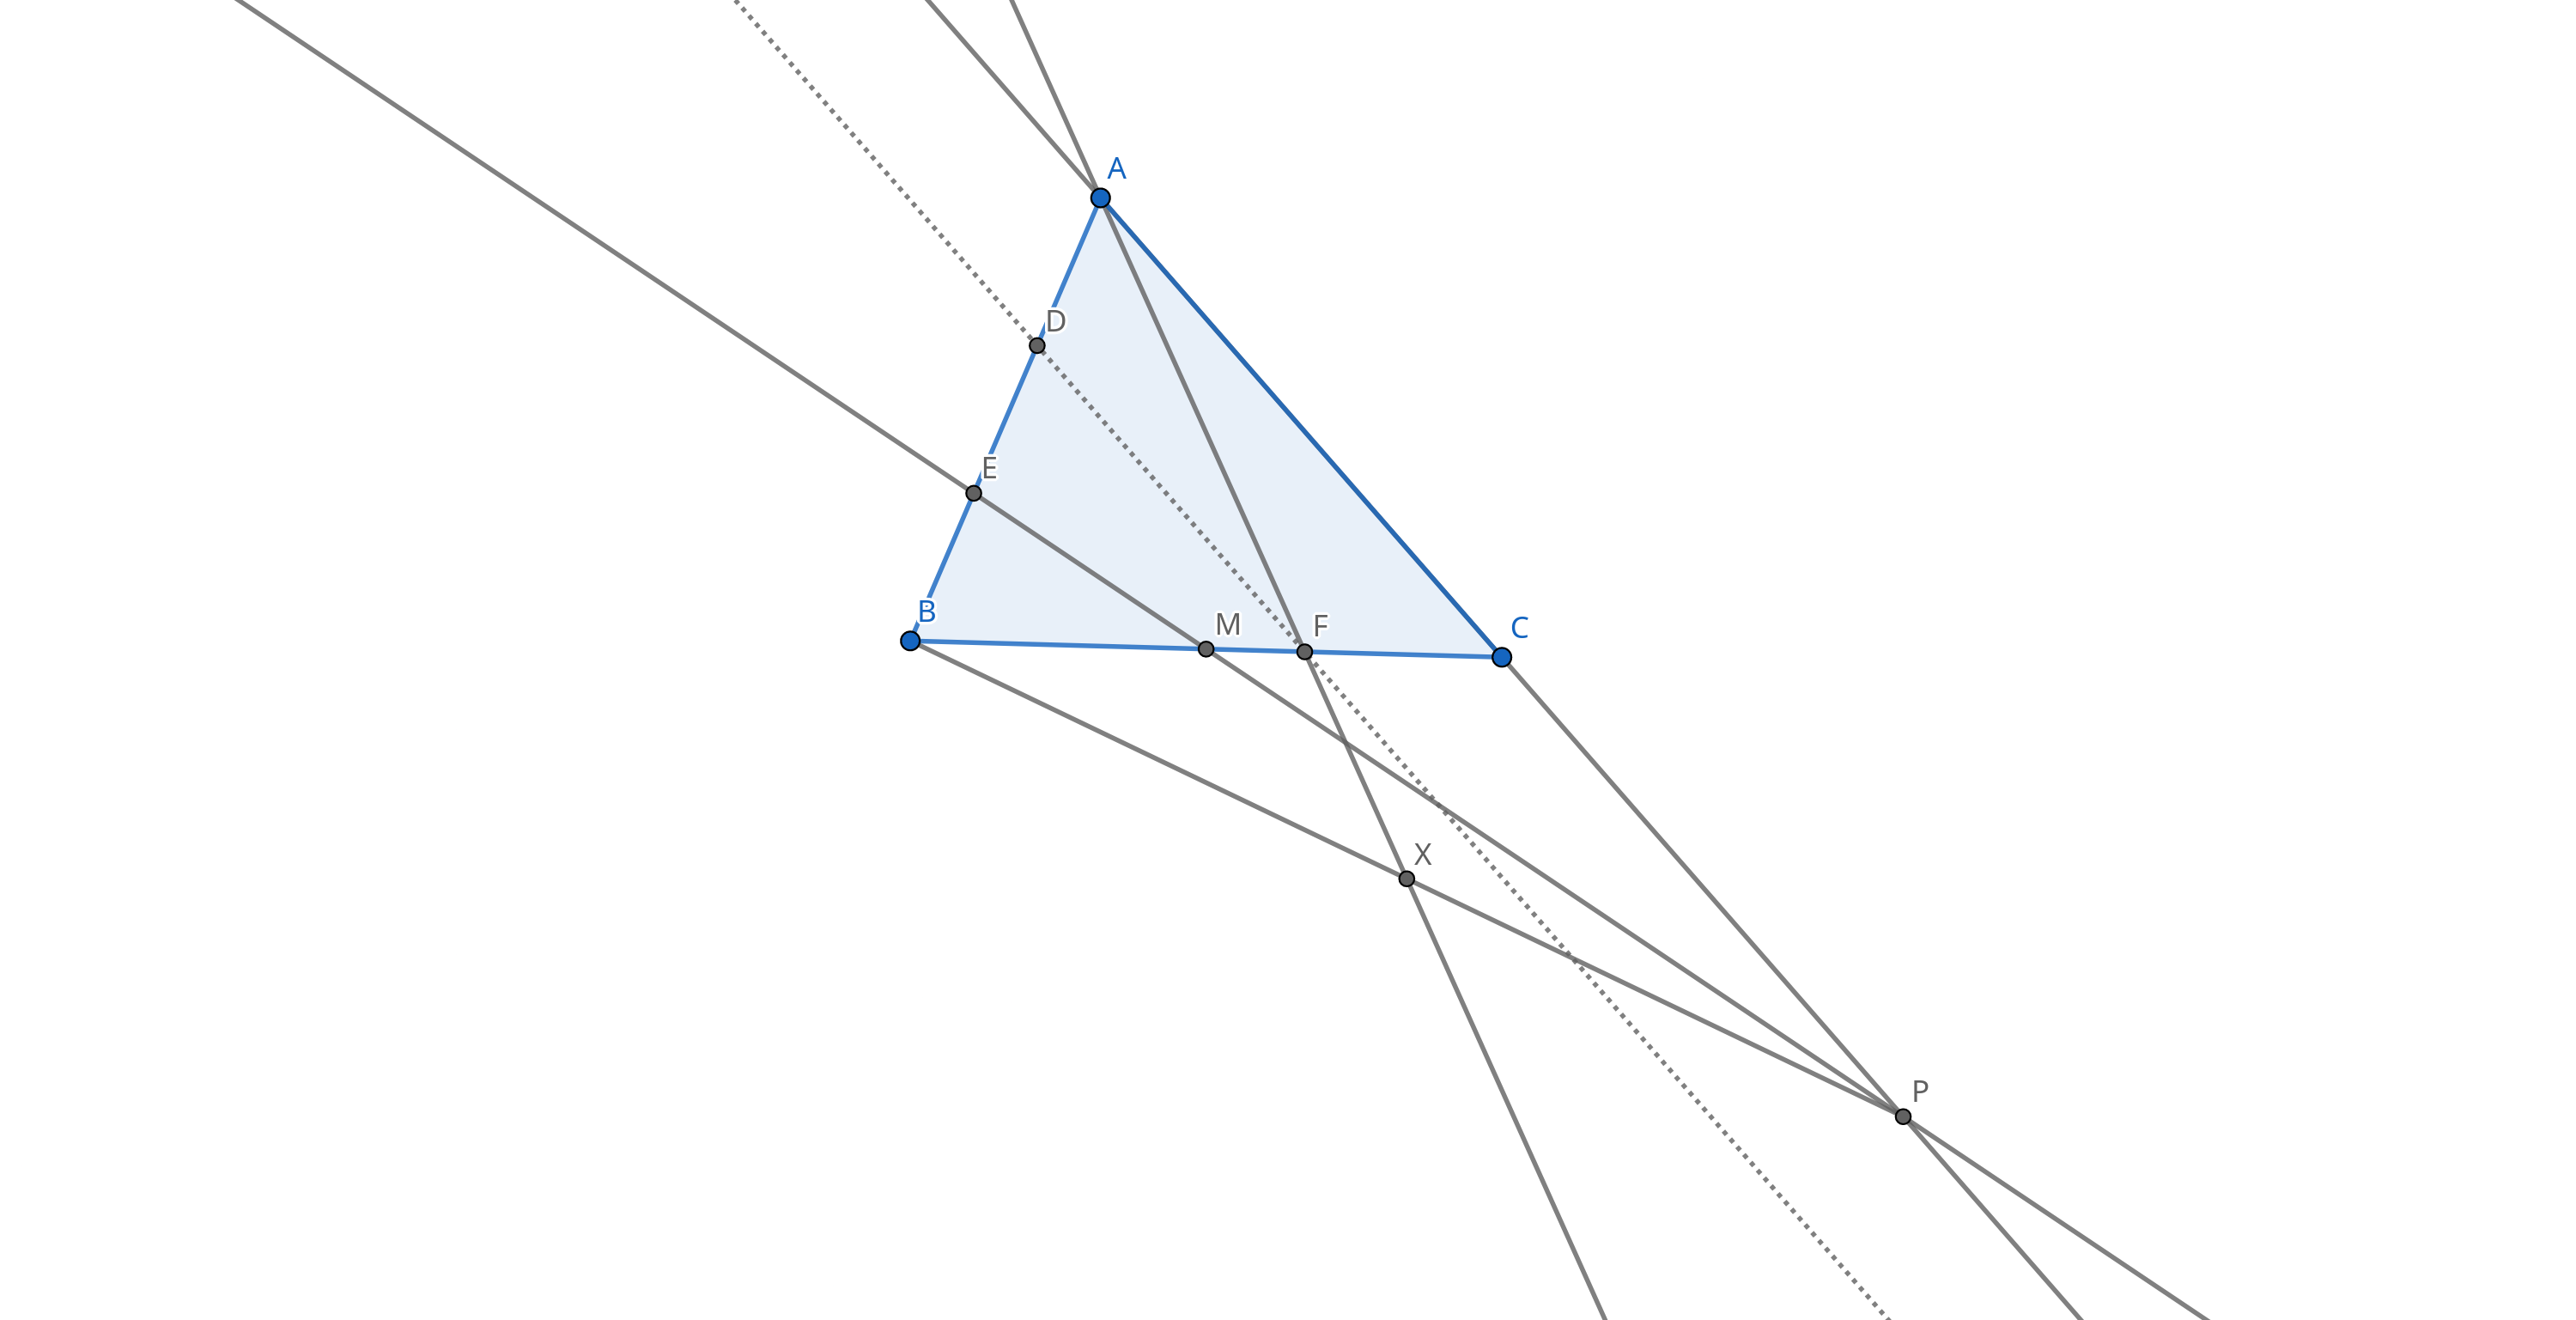
\includegraphics[width=0.95\textwidth]{1-fig.png}
  \end{center}
  \caption{Konstrukce}
  \label{fig:1}
\end{figure}


Ze zadání můžeme snadno odvodit, že $D = (2 : 1 : 0)$, $E = (1 : 2 : 0)$
a $M = (0 : 1 : 1)$. Díky podobnosti trojúhelníků $ABC$ a $ADF$ rychle
odvodíme, že $\frac{|BD|}{|DA|} = \frac{|BF|}{|FC|}$, proto tento bod
$F = (0 : 1 : 2)$. Následně abychom zjistili bod $P$, vyjádříme si
přímku $EM$:

\[
  u + 2v = 0
\]
\[
  v + w = 0
\]

Obecná rovnice přímky $EM$ je tedy:

\[
  2x - y + z = 0
\]

Z toho jsme schopni zjistit souřadnice bodu $P$:

\[
  2x - y + z = 0
\]
\[
  y = 0
\]
\[
  x + y + z = 1
\]

Souřadnice tedy jsou $P = (-1 : 0: 2)$.

Teď vyjádříme přímku $AF$:

\[
  u = 0
\]
\[
  v + 2w = 0
\]

Takže obecná rovnice přímky $AF$ je:

\[
  2y - z = 0
\]

Když do toho dosadíme střed úsečky $BP$, získáme:

\[
  2 \cdot \frac{1 + 0}{2} - \frac{2 + 0}{2} = 1 - 1 = 0
\]

Tudíž střed úsečky $BP$ leží na přímce $AF$, což jsme chtěli ukázat.


\end{document}
